\chapter{Introduction}

\begin{center}
  \textit{There is no other species on the Earth that does science. It is, so 
    far, entirely a human invention, evolved by natural selection in the 
    cerebral cortex for one simple reason: it works.}

 - Carl Sagan
\end{center}

\section{Protein NMR}
NMR (Nuclear Magnetic Resonance) spectroscopy is an experimental technique for 
studying proteins and other biological molecules at atomic resolution.  In 
comparison to other techniques for high-resolution characterization of 
biological molecules, NMR's significance as an experimental technique stems 
from its ability to collect detailed molecular data, from which further 
analysis can derive not only structural information but also dynamics, 
activity, and interactions with other molecules.  The importance of NMR 
spectroscopy to the structural biology community has steadily increased, as 
measured by the number of biologically relevant molecules that have been 
studied using the technique, and the corresponding data deposited into 
publicly available databases -- since 1990, the structures of nearly 9,000 
proteins that were solved using NMR have been deposited in the Protein Data 
Bank (PDB) \cite{pdb}, a facility for the archival and sharing of protein-related 
data, and NMR data is available for over 10,000 proteins in the BioMagnetic 
Resonance Bank (BMRB) \cite{bmrb}, a facility for the archival and sharing of 
specifically NMR-derived data.  The data collected using NMR techniques is 
important to the field of drug design 
\cite{stockman2002drugs, moore2003leveraging, reckel2011proteorhodopsin}, 
as it facilitates identification of potential 
binding partners based on surfaces as well as actual binding partners based on 
chemical shifts, and understanding biological processes.




\section{Scientific Methods and Reproducibility}
The term "science" can refer to both the enterprise of knowledge acquisition 
through empirical means, and the body of knowledge acquired through such means 
\cite{drummond2012reproducible}.
The core of science is the notion of reproducibility 
\cite{russell2013reproducibility, nih2014reproducibility} -- that claims can be 
independently tested and verified.  Reproducible knowledge can be 
obtained using a set of general techniques collectively known as "the 
scientific method".  These techniques share many characteristics, most notably:
\begin{itemize}
 \item data collection: observation of a natural phenomenon, in which 
 experiments are performed and the results quantified and recorded
 \item analysis, in which the data collected in an experiment is processed to 
 gain information, knowledge, and understanding
 \item experimental design: inventing and codifying a procedure for data 
 collection which tests specific variables of a system, while preventing 
 other variables from confounding the results
 \item hypotheses, which synthesize and organize the information, knowledge, 
 and understanding gained in order to both explain the observed results and 
 predict the outcomes of further experiments
\end{itemize}

Reproducible research is the combination
of a scientific result, along with the data, experiments, and analyses used 
to obtain that result, in sufficient detail such that an indepdendent researcher
could, in principle, perform the same produce and reach the same result.

Two example orderings of these basic steps are shown in 
Figure \ref{scientific_method_pipeline}, in which a rigid structure is
imposed as a sequential pipeline, and Figure \ref{scientific_method}, which 
is a more flexible method because it allows any step to influence any other 
step.  In general, as both examples illustrate, the core of science is a
method of iterative experimental designing, data collection, analysis, and 
hypothesis formulation, which leads to new experiments, data and analysis,  
and so on, resulting in the acquisition of knowledge about the natural world.

A basic principle of scientific methods is that they enable reproducibility.  
In order for scientific results to be reproducible, all components of the 
experimental design, data collection and data analysis steps must be 
reproducible.  These include:
\begin{itemize}

  \item Experimental design.  Our understanding of scientific methods, the 
  significance of reproducibility, and means of achieving reproducibility 
  have evolved along with our experimental methods.  
  Lab notebooks are a standard tool for recording information.  Their 
  advantages are well-known \cite{rubacha2011eln}: not only do they enable 
  flexible and persistent storage of information, they also enhance 
  continuity within research groups as personnel, techniques, 
  and reagents change over time by explicitly recording key information.
  Experimental designs must be recorded in sufficient detail to convey the key
  points to other scientists.  It may also acknowledge the possibility of 
  confounding variables, and take measures to control for them.
  The appropriate level of detail is neither too much nor too little:
  it should be repeatedly executable such that similar results are obtained 
  -- within expected deviations due to experimental error and variables 
  outside the control of the experiment \cite{drummond2012reproducible}.
  The long history of usage of lab notebooks has created a rich culture of
  their use; scientists have a well-developed understanding of what should,
  and what should not, be recorded.

  \item Experimental execution.  Lab notebooks and Laboratory Information 
  Management Systems 
  (LIMS) are also important for recording the details of experiments, including 
  any problems such as contamination.  Recent efforts have applied 
  computational power to create Electronic Lab Notebooks (ELNs)
  \cite{talbott2005eln, rubacha2011eln, myers2001eln}.
  Previous efforts led to results such as Good Laboratory Practices (GLPs) and
  Good Manufacturing Practices (GMPs), intended to ensure quality and
  reproducibility within industry research and manufacturing efforts
  \cite{macleod2008reprint, unger2008good}.
  When carrying out an experiment, the actual procedure followed should be
  recorded in sufficient detail, including any deviations from the given 
  experimental design and justifications for those changes.
  Biased sampling should also be recognized if possible
  \cite{savovic2012influence, simmons2011false}.
  Journal publications are used to convey information about experimental
  designs and results to other scientists.  Scientists thus have a firm
  notion of experimental reproducibility.

  \item Computational.  As computers continue to play an ever-growing role in 
  science, scientists have noted the problems that indiscriminate computational 
  use poses for reproducibility \cite{donoho2009, peng2011reproducible}.  
  By the early 1990's, researchers began defining reproducible 
  computational analysis \cite{donoho_wavelab}, and describing strategies for 
  achieving it.  A key point is that all tools, scripts, platforms and code 
  available, including the exact versions used
   \cite{ince2012open, nekrutenko2012next, blankenberg2014dissemination}.
  In addition, all parameterizations \cite{landis2012call}, as well
  as input and output data should be recorded.

  \item Analysis.  A further concern of reproducibility is with 
  non-computational analysis; failing to recognize analytical bias and to 
  use appropriate statistical measures has long been a source of 
  irreproducibility in scientific endeavors \cite{sackett1979bias}.
  This has also been previously noted in \cite{ioannidis2005most} 
  in \cite{nuzzo2014statistical, begley2013reproducibility}, 
  and was the focus of a recent Nature special 
  (\url{http://www.nature.com/nature/focus/reproducibility/}).
  To ensure reproducibility of analysis, appropriate, necessary, and sufficient
  statistical measures should be used
  \cite{pashler2012replicability, vaux2012numbers}.
  If bias is present in the experimental data, its sources should be recognized
  and accounted for \cite{macarthur2012reproducibility, wagenmakers2012agenda}.
  Additionally, manual changes made during analysis should be recorded.

\end{itemize}

Reproducibility is important to science for several reasons 
\cite{borgman2012conundrum}.  First, it 
provides a means for measuring the quality and usefulness of a study or 
claim.  Second, reproducibility facilitates knowledge transfer between 
peers, which enables fellow researchers to build on the foundation provided 
by a study, whether by extending the experimental design and data collection, 
applying the experiment in a different context, or applying additional analyses 
to existing data.  Third, reproducibility promotes collaboration between fellow 
scientists by enabling sharing of data \cite{rung2013reuse}, 
information, knowledge and experimental 
designs.  Fourth, reproducibility reduces time wastage due to inability to 
replicate results 
\cite{ioannidis2005most, mullard2011reliability, prinz2011reproducibility,
begley2012drug}. 


\section{Irreproducibility of computational and manual analysis in NMR}
Much progress has been made within NMR in the areas of experimental
reproducibility and their dissemination.  In addition, many software tools
exist for structure validation \cite{doreleijers2012nrg, laskowski1996aqua, bhattacharya2007evaluating}.
Tools such as ShiftX2 \cite{shiftx2}, which use final results to back-predict
intermediate data, also provide consistency checks which are useful for
evaluating reproducibility.  The BMRB's efforts to model, archives, and 
disseminate NMR-obtained data and results are critical to efficient sharing of
techniques and results between NMR spectroscopists.

However, computational results are often irreproducible due to missing code and data;
additionally, strategies for computational reproducibility covering all 
uses of computation are not yet in place despite efforts such as 
\cite{donoho2009, peng2011reproducible}.
Sequential, deductive processes pose different challenges for reproducibility,
as strategies for efficiently capturing the full set of information in a 
meaningful and easy-to-understand way continue to be elusive.  Integration
of manual analysis with computational analysis poses further unsolved
challenges for reproducibility.

Thus, this work will focus on the irreproducibility of computational and manual
analysis in the field of NMR protein structure determination.
The context of NMR will be explored from a data-centric standpoint, as well as
the process of analysis and its interaction with the data.
This will be used to demonstrate that NMR data analysis, both computational
and manual, is not reproducible
because of several broad categories of data which are not explicitly 
recorded during the analysis process and are lost.


\section{The significance of reproducibility to NMR}
Irreproducible NMR spectral analysis and structure determination causes 
several problems.  The value and 
quality of irreproducible NMR analyses are difficult or impossible to judge; 
irreproducibility limits the ability to transfer knowledge and techniques 
(for interpretation of spectra, resonance assignment, stereospecific resonance 
assignments, etc.) effectively between scientists, as well as preventing close 
collaborations during data analysis and leading to time wastage as 
irreproducible results are discovered and following up on them is found to be 
impossible.  In addition, irreproducibility renders error detection and 
correcting difficult, because the data that would show when, why, and how an 
error occurred would be lost.  It also causes the teaching of analysis methods 
to students and other newcomers to be difficult due to implicit, missing data; 
by capturing and making explicit these data, a more complete picture of the 
process can be discussed and shown.  Finally, irreproducible data may be less 
amenable to future reinterpretation; reinterpreting data is necessary when 
augmenting a data set with additional results, which may fill in missing 
pieces, but may also show the original analysis to be in error.  In short, 
reproducibility of NMR spectral analysis and structure determination will lead 
to better quality results.


\section{An Approach for Reproducible Analysis}
One possible approach for rendering analysis reproducible will be discussed.
The limitations of current practices in capturing insufficient data are 
covered, and a data model for the additional information is presented.
Then, a general strategy for using the data model is described.
Additionally, this section will discuss how to effectively put this strategy 
into practice, covering common roadblocks and problems as well as tips and 
suggestions.


\section{Reproducible NMR Data Sets}
In order to prove the utility of the reproducibility approach and annotation 
model in practice, it was applied to a full-scale protein structure 
determination process.  Starting with time-domain data sets of the protein of 
interest, the structure determination process was carried out from start to 
finish, including peak-picking, sequence-specific assignment, NOESY analysis 
and structure calculation.  Intermediate snapshots were captured and 
appropriately annotated.  This data set may now be found deposited in the BMRB.

The data model used was based on the data models of the CCPN project \cite{ccpn}
and of the BMRB \cite{bmrb}, with several 
extensions as previously noted to enable reproducibility.  A library of NMR 
phenomena and their use as deductive inferences rules was constructed.  
These rules were applied for snapshot annotation.

Whereas a single implementation of the previously described strategy is 
here described, in principle the approach is platform-agnostic and 
therefore could be implemented and used by other research group, or added 
into an existing tool as an extension.


\section{Software for Practical Reproducibility}
Software tooling comprises a significant portion of enabling practical 
reproducibility.  High-quality tools can make reproducibility easy, pleasant, 
and safe (in the sense of not error-prone), without placing additional 
unreasonable time, effort, and education demands on potential users.  This 
section will explore a suite of software designed to enable and support 
reproducibility of NMR analysis in various ways.
	
First, a Sparky reproducibility extension has been developed.  This extension
facilitates reproducible data capture during the spectral analysis stage. Sparky 
\cite{sparky} is a popular tool for analysis of NMR data.  One of the major 
strengths of Sparky is its extensibility through user-defined Python modules.  
While its core is written in C++ and is not extensible, a Python module can 
be added without needing to touch the C++ core.  This extension allows
simple data snapshotting, annotation, and capture of extraneous results,
without disrupting the standard Sparky user experience.  The increase in
workload is minimal due to Sparky's keyboard accelerators.

Second, a library for reading and writing of NMR-STAR files was implemented.  
NMR-STAR is the standard format used by the BMRB for the deposition and 
archival of NMR data \cite{hall1991star, hall1994star, hall1995star}.
By storing ongoing data analysis in NMR-STAR files, 
users gain the benefits of data integration with the BMRB -- analysis results 
can be uploaded and thereby shared with fellow researchers.  The approach 
taken in implementing and using this parser represents a radical departure 
from standard NMR software techniques; the approach ensures that the 
software will remain easily usable and maintainable as NMR data expands 
and matures.

Third, two tools for working with time- and frequency-domain data sets:  
Connjur Spectrum Translator (ST) and Connjur Workflow Builder (WB).  ST 
translates between various formats of time- and frequency-domain spectra; 
such a tool is necessary because of the input and output requirements of 
many spectral processing tools.  WB provides a high-level interface to 
spectral processing and stores the parameterization, functions, and 
intermediate data sets in a central, relational database.  This means 
that the stage is reproducible.

Fourth, a sample scheduler has been implemented.  This tool facilitates the 
creation of non-uniform sample schedules, which are used to collect time-domain 
data which are non-uniformly sampled in the indirect dimension(s).  Non-uniform 
sampling can help decrease the amount of data collection time required, and 
also help in avoiding the penalties imposed by the necessity of sampling past 
the Rovnyak limit \cite{rovnyak2004accelerated}.  This project included,
a novel data model of sample schedules which included non-uniformity not 
only in the time dimensions but also in the number of transients per FID and 
the quadrature, 
a collection of common algorithms, gathered from descriptions in the 
literature and implemented,
and facilitated easy reproducibility of sample schedule creation by capturing
the parameterization.


\section{CONNJUR is Free and Open Source}
All software developed by the CONNJUR team is released under standard open 
source licenses and is freely available on our website.  The open source 
movement first became popular as a means for users to get control and legal 
rights over software that they had purchased.  This level of ownership is 
important because it enables users to freely and perpetually use, share, 
inspect, fix, maintain, and improve their software.  Such considerations 
become important in view of the rapid changes that scientific fields -- 
including NMR -- undergo: new datatypes, analyses, statistical measures, 
and protocols are developed, requiring updates to old software or entirely 
new software to be written from scratch.  Open source software provides 
additional value in the context of reproducibility: in order to replicate a
study, one must have access to the exact same computational tools that the 
original study used \cite{ince2012open}.  
This involves both physical access -- in the sense of 
being able to get a program loaded onto a computer -- as well as licensing 
issues: does the second group have the rights to use the software in the 
exact same way as in the original study.

Our belief is that open source software can help mitigate these and other 
problems, as well as aid the field in more effectively dealing with its 
nascent software problem, by leading to adoption of a community development 
model and increased sharing, reducing the barriers to future progress in 
the field.  We can only hope that other research groups place as much value 
as we do on open source licenses, and that adoption of open source development 
models will increase.  


\section{Scope and Significance}
Reproducibility is a key enabler of the success of the scientific approach to 
acquiring knowledge.  This work inspects reproducibility in the field of NMR, 
defines the requirements for data analysis that must be met in order to achieve 
reproducibility, and identifies where current practices fall short.  To remedy 
this situation, a strategy for reproducible data analysis is presented.  This 
strategy is made practical by means of a formal model, support from the BMRB 
\cite{bmrb}, and a software implementation.

Reproducibility of analysis offers additional potential benefits.  By making
the data involved in the process explicit, it facilitates communication and
reveals bias.  Both advantages can lead to major improvements in the quality
of NMR analysis.  Improved communication helps the transfer of knowledge
between scientists, which is useful for building on established protocols
and techniques, as well as for teaching and learning.  Revealing sources of
bias highlights the deficiencies of current practices, indicating areas 
which would most benefit from improvements.  Therefore, improving the 
reproducibility will lead to improvements in quality as well.


% figures
\clearpage
\section{Figures}

\begin{figure}[h]
  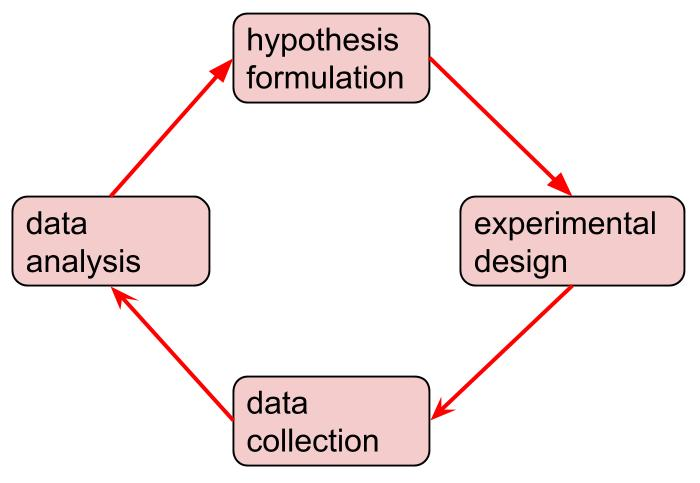
\includegraphics[scale=0.5]{figures/scientific_method_pipeline}
  \caption{A scientific method as a sequential, cyclic pipeline}
  \label{scientific_method_pipeline}
\end{figure}

\begin{figure}
  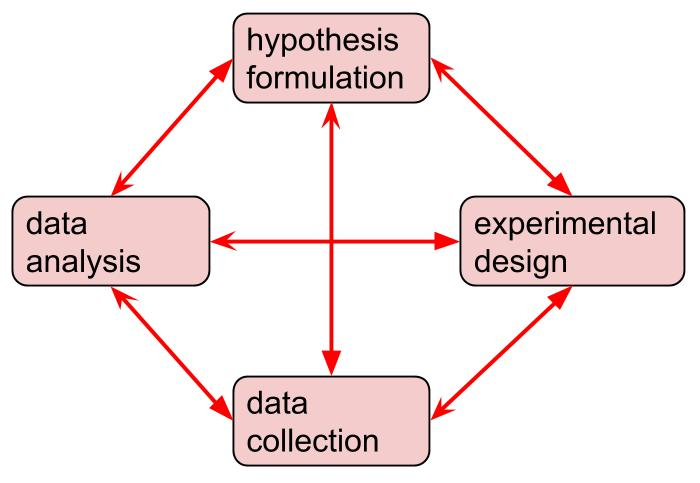
\includegraphics[scale=0.5]{figures/scientific_method}
  \caption{A scientific method in which each step interacts with every other}
  \label{scientific_method}
\end{figure}

